\documentclass[12pt, a4paper]{article}

\usepackage{graphicx}
\usepackage{amsmath}
\usepackage{algorithm}
\usepackage{algpseudocode}
\usepackage[margin=3cm]{geometry}
\usepackage{algcompatible}



\begin{document}

\tableofcontents
\newpage

\section{Problem 1 : Introduction}
\subsection{Description}

F5 : $ab^x$ is an exponential function, where a is a constant value, $a \ne 0$ and it also represents starting (initial) value , b is called base and is a positive real number and $b \ne 1$, x is called the exponent (power), it is independent variable . In this function, b is a constant value, whereas x is variable.

\subsection{Domain}

The domain for exponential function is the set of real numbers. 
\newline $x \in R$ ,  -$\infty < x <\infty$ , Domain : $\{x \mid x \in R$\}

\subsection{Co-Domain}

Co-Domain is the set of all possible function output values.
\newline Suppose $y = f(x) = ab^x $, then -$\infty < y <\infty$ , so the range will be $[-\infty,\infty]$.

\subsection{Characteristics}
\begin{itemize}
    \item In exponential function, if $ b > 0 $, then it is known as exponential growth function (increasing function). Its graphical representation shown in the left part of the figure 1.
    \item In exponential function, if $ 0 < b < 1$, then it is known as exponential decay function (decreasing function). Its graphical representation shown in the right part of the figure 1.
    \item Exponential function have horizontal asymptote (i.e function approaches to a imaginary horizontal line but never crosses) at $ Y=0 $ (i.e $ X $ – axis).
    \item They are continuous function.
    \item There is no symmetry in exponential function, so they are neither odd nor even function.
    \item Exponential function is not injective but is surjective. 
\end{itemize}

\newpage

\begin{figure}[h]
  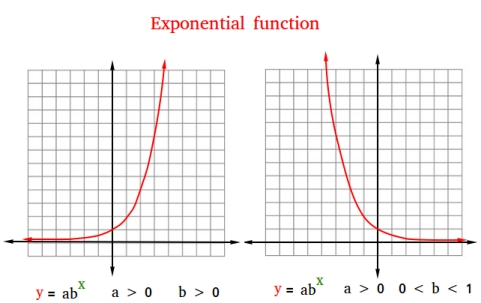
\includegraphics[width=\linewidth]{exponential-function.jpg}
  \caption{Exponential Function Graph (Growth And Decay).}
  \label{fig:exponential function graph (growth and decay)}
\end{figure}

\subsection{Context of Use Model}
\begin{figure}[h!]
  
\includegraphics[width=0.5\linewidth]{frog.jpg}
  \caption{Exponential Function Graph (Growth And Decay).}
  \label{fig:exponential function graph (growth and decay)}
\end{figure}


\newpage

\section{Problem 2 : Requirements}
\begin{enumerate}
    \item{} Requirement 1
        \begin{itemize}
        \item \textbf{ID} : REQ1
        \item \textbf{Version} : 1.0
        \item \textbf{Type} : Functional Requirement
        \item \textbf{Priority} : High
        \item \textbf{Difficulty} : Easy
        \item \textbf{Description} : In the exponential function $ ab^x $, the input value a should be greater than 0 i.e., $ a > 0 $ (or else it will result in output of the function to be 0 for every input), also input value of base b must be greater than 1 i.e., $ b > 1 $ (or else if $b = 1 $, it will result in output of the function to be ‘a’ for every input of x).
        \end{itemize}
    
    \item{} Requirement 2
        \begin{itemize}
        \item \textbf{ID} : REQ2
        \item \textbf{Version} : 1.0
        \item \textbf{Type} : Functional Requirement
        \item \textbf{Priority} : High
        \item \textbf{Difficulty} : Easy
        \item \textbf{Description} : In the exponential function $ab^x$, the input value of base b must not be negative as it will result will be complex numbers so $b > 0$.
        \end{itemize}
    
    \item{} Requirement 3
        \begin{itemize}
        \item \textbf{ID} : REQ3
        \item \textbf{Version} : 1.0
        \item \textbf{Type} : Functional Requirement
        \item \textbf{Priority} : High
        \item \textbf{Difficulty} : Easy
        \item \textbf{Description} : In the exponential function $ab^x$, the input value of x must be any real number. i.e $x \in R$.
        \end{itemize}
    
    \newpage
    
    \item{} Requirement 4
        \begin{itemize}
        \item \textbf{ID} : REQ4
        \item \textbf{Version} : 1.0
        \item \textbf{Type} : Functional Requirement
        \item \textbf{Priority} : High
        \item \textbf{Difficulty} : Medium
        \item \textbf{Description} : The system must take input values of a, b and x from the users and return the output of $ab^x$ function. For example, if $ a = 2, b = 3 , x = 2,$ the output should be $ 18 $.
        \end{itemize}
    
    \item{} Requirement 5
        \begin{itemize}
        \item \textbf{ID} : REQ5
        \item \textbf{Version} : 1.0
        \item \textbf{Type} : Functional Requirement
        \item \textbf{Priority} : High
        \item \textbf{Difficulty} : Easy
        \item \textbf{Description} : If any of the input values a, b or x are not provided by the user, the system should not accept that input and ask user to provide the missing values. 
        \end{itemize}
    
    \item{} Requirement 6
        \begin{itemize}
        \item \textbf{ID} : REQ6
        \item \textbf{Version} : 1.0
        \item \textbf{Type} : Functional Requirement
        \item \textbf{Priority} : High
        \item \textbf{Difficulty} : Easy
        \item \textbf{Description} : If the input values are not of integer type, the system must not accept it and handle the error and ask for integer values as input.
        \end{itemize}
        
    \newpage
    
    \item{} Requirement 7
        \begin{itemize}
        \item \textbf{ID} : REQ7
        \item \textbf{Version} : 1.0
        \item \textbf{Type} : Functional Requirement
        \item \textbf{Priority} : Medium
        \item \textbf{Difficulty} : Easy
        \item \textbf{Description} : If the user enters any large input value which the system cannot handle, it should throw an exception and handle it accordingly.
        \end{itemize}
     
    \item{} Requirement 8
        \begin{itemize}
        \item \textbf{ID} : REQ8
        \item \textbf{Version} : 1.0
        \item \textbf{Type} : Non-Functional Requirement
        \item \textbf{Priority} : High
        \item \textbf{Difficulty} : Medium
        \item \textbf{Description} : The computation of the function must be performed within some desired time to provide better performance.

        \end{itemize}
    
\end{enumerate}

\newpage

\section{Problem 3 : Algorithms}

Two algorithms (Algorithm 1 and Algorithm 2) have been selected for \newline
implementing the function $y = ab^x $. The pseudocode for each of the algorithm is provided in this section followed by their detailed description and the advantages as well as the disadvantages of each approach are discussed later.

\subsection{Algorithms and Pseudocode}
\begin{algorithm}[hbt!]
\caption{Iterative-Exponent(a,b,x)}\label{alg:one}

\hspace*{\algorithmicindent} \textbf{Input : }double number $a,b,x$ \\
\hspace*{\algorithmicindent} \textbf{Output : }value of the function $ab^x$ represented by double number result
\begin{algorithmic}[1]
\STATE $temp \gets 1$
\WHILE{$x > 0$}
  \STATE $temp \gets temp \times b$
  \STATE $x \gets x - 1$
\ENDWHILE
\STATE $result \gets a \times temp$
\STATE return $result$
\end{algorithmic}
\end{algorithm}

In this algorithm, the iterative approach is used for calculation of the given function, $ab^x$, Initially a temporary  variable called $temp$ is initialized to 1 and to calculate $b^x$, While loop is used for all the values of $x$ (exponent) and in each iteration, $temp$ is multiplied by $b$ (base) and the value of $x$ is decremented by 1. The loop continue until the exponent value $x$ reaches to 0. At last, $a$ is multiplied with the $temp$ value $(a*b^x)$ and the output is obtained in the result and it is returned.

\vspace{40mm}


\begin{algorithm}[hbt!]
\caption{Recursive-Exponent(a,b,x)}\label{alg:two}

\hspace*{\algorithmicindent} \textbf{Input : }double number $a,b,x$ \\
\hspace*{\algorithmicindent} \textbf{Output : }value of the function $ab^x$ represented by double number result
\begin{algorithmic}[1]
\STATE $temp \gets recursive\_power(b,x)$
\STATE $result \gets a \times temp$
\STATE return $result$
\end{algorithmic}
\end{algorithm}

\newpage


\begin{algorithm}[hbt!]
\caption{recursive\_power(b,x)}\label{alg:two}

\hspace*{\algorithmicindent} \textbf{Input : }double number $b,x$. \\
\hspace*{\algorithmicindent} \textbf{Output : }value of $b^x$ will be returned.
\begin{algorithmic}[1]
\IF{$x \neq (Integer) x $}
  \STATE return $ fraction\_power(b,x) $
\ENDIF
\STATE $helper \gets recursive\_power(b,x/2)$
\IF{$x < $ 0}
  \STATE $ b  \gets $ 1.0/$ b $
  \STATE $ x  \gets  - x $
  \IF{$x$ mod 2 = 0}
  \STATE return $helper \times helper$
  \ELSE
  \STATE $x \gets x - 1$
  \STATE return $helper \times helper \times b$
\ENDIF
\ELSIF{$x$ = 0}
  \STATE return $1.0$
\ELSIF{$x$ = 1}
  \STATE return $b$
\ELSIF{$x$ mod 2 = 0}
  \STATE return $helper \times helper$
\ELSE
  \STATE $x \gets x - 1$
  \STATE return $helper \times helper \times b$
\ENDIF
\end{algorithmic}
\end{algorithm}

In this algorithm, the recursive approach using divide and conquer strategy is used for the calculation of the given function $ab^x$. $recursive\_power(b,x)$ algorithm is used for calculating the value of $b^x$, the recursive call to the function with value base $b$ and $x = x/2$ i.e $recursive\_power(b,x/2)$ is stored in helper, so that it needs to be computed just once and can be used later on. If the value of exponent $x$ is fractional, it is checked and $fraction\_power(b,x)$ will compute all the power values of such exponents. For negative value of exponent, value of base $b$is reciprocated and that of exponent $x$ is negated and on the basis of the parity the algorithm performs the computation. In the base case, if the value of $x$ is 0, value $1$ is returned, otherwise, if $x=1$, value $b$ is returned, if the exponent is divisible by $2$, the algorithm recurses on $(helper * helper)$ and for odd value of exponent, the value of exponent is decremented by $1$ and then it recurses on $(helper * helper * b)$,  At last, $a$ is multiplied with the returned value from $recursive\_power(b,x)$ and the output is obtained in the $result$, and it is returned.

\newpage
\begin{algorithm}[hbt!]
\caption{fractional\_power(b,x)}\label{alg:two}

\hspace*{\algorithmicindent} \textbf{Input : }double number $b,x$. \\
\hspace*{\algorithmicindent} \textbf{Output : }value of $b^x$ will be returned.
\begin{algorithmic}[1]
\STATE $exponentValue \gets 0$
\STATE $iterations \gets 150$
\STATE $logValue \gets logarithm\_calculator(b)$
\WHILE{$iterations >= 0$}
  \STATE $powerValue \gets recursive\_power((x * logValue) , iterations) $
  \STATE $factorialValue \gets factorial\_calculator(iterations)$ 
  \STATE $exponentValue \gets exponentValue + (powerValue / factorialValue)$
  \STATE $iterations \gets iterations - 1$
\ENDWHILE

\STATE $reciprocalExponentValue \gets 1/exponentValue $
\IF{$x > $ 0}
  \STATE return $exponentValue$
\ELSE
 \STATE return $reciprocalExponentValue$
\ENDIF

\end{algorithmic}
\end{algorithm}
\vspace*{-.4cm}
\begin{algorithm}[hbt!]
\caption{logarithm\_calculator(n)}\label{alg:two}

\hspace*{\algorithmicindent} \textbf{Input : }double number $n$. \\
\hspace*{\algorithmicindent} \textbf{Output : }natural logarithmic value of n $ln(n)$ will be returned.
\begin{algorithmic}[1]

\STATE $iterations \gets 100$
\STATE $logValue \gets 0 $
\IF{$n < $ 0}
  \STATE $n \gets -n$
\ENDIF
\STATE $baseValue \gets (n - 1) / (n + 1) $

\WHILE{$iterations > 0$}
  \IF{$iterations$ mod $2 \neq 0$}
  \STATE $logValue \gets logValue + recursive\_power(baseValue , iterations) / iterations $
  \ENDIF
  \STATE $iterations \gets iterations - 1$
\ENDWHILE
\STATE return $logValue * 2$

\end{algorithmic}
\end{algorithm}

\begin{algorithm}[hbt!]
\caption{factorial\_calculator(n)}\label{alg:two}

\hspace*{\algorithmicindent} \textbf{Input : }double number $n$. \\
\hspace*{\algorithmicindent} \textbf{Output : }factorial value of $n$ will be returned.
\begin{algorithmic}[1]

\IF{$n = $ 0}
  \STATE return $1$
\ENDIF
\STATE return $ (n * factorial\_calculator(n-1)) $

\end{algorithmic}
\end{algorithm}



\newpage
Algorithm $fractional\_power(b,x) $ helps in finding the power of any fractional exponent, the given exponent and base are converted as, $b^x = (e^{ln(b)})^x = e^{xln(b)} $, where the natural logarithm value for b is computed using the $logarithm\_calculator(n) $ algorithmFinally, the computation of $e^{xln(b)} $ is performed by calculating numerator(powerValue) by using $recursive\_power$ , passing $x * value of ln(x) $ as base and $iteration \hspace{1mm} number$ as exponent and the denominator is the factorial value of the iteration number obtained using the $factorial\_calulcator(n)$ algorithm, numerator and denominator are divided and their result is stored in the $exponentValue$ which is returned after completion of all the given number of iterations.

\subsection{Advantages and Disadvantages}



\subsubsection{Algorithm 1}
Iterative Approach

Advantages:
\begin{enumerate}
    \item {Iterative algorithms are simple and easy to develop; they can be easily understood by the reader.}
    \item {In Iterative approach there is no overhead of function calls and they do not use stack memory and hence don’t suffer from stack overflow.}
    
\end{enumerate}

Disadvantages:
\begin{enumerate}
    \item {Some iterative algorithms are slower when compared to other approaches, Algorithm 1 which was described previously has time complexity of O(n) , so for larger inputs it is inefficient.}
    \item {If the termination condition of control variable is not defined properly, it may lead to infinite loop.}
    
\end{enumerate}

\subsubsection{Algorithm 2}
Recursive Approach 

Advantages:
\begin{enumerate}
    \item {Recursive Algorithms have less time complexity for certain problems;  Algorithm 2 which was described previously has time complexity of $O(logn)$ which is better than that of Algorithm 1.}
    \item {Recursive Algorithms are very useful in situations where particular solution is to be applied repeatedly.}
    
\end{enumerate}

Disadvantages:
\begin{enumerate}
    \item {Recursion is more difficult to understand in some algorithms and tracing them is difficult}
    \item {Recursive algorithms utilize too much memory and when the base case is not defined properly it may lead to infinite loop or crashing of the CPU.}
    
\end{enumerate}

\subsection*{Decision}
Algorithm 2 (recursive approach) would be a better option for the implementation of the function $ab^x$ as it has lower time complexity and the computation of the function must be performed quickly, so it is preferable to use the recursive algorithm rather than the iterative algorithm.
\newpage

\section{Problem 4 }
\subsection{Debugger}
\subsubsection{Description}
Debugging provides the facility for identifying and eliminating bugs, errors present in the program. This process can help in tracing the reasons behind the improper functional behaviour of any program. For debugging, I have used the IntelliJ debugger tool for java language and depending on the various installed plugins, it provides support for debugging code in different languages as well. IntelliJ debugger allows the facility to run the program step by step and keep a track of the values of the associated variables.

\subsubsection{Advantages : }
\begin{enumerate}
    \item Breakpoints are special kind of markers which when encountered the debugger temporarily halts the program execution (suspended program state) and it makes easier to analyse and debug those special lines.
    \item It allows to trace the values of the variable throughout the program, such trace would be helpful to identify the points where the incorrect values are assigned to the variables, also it provides information about the status of the threads.
    \item It enables execution of any arbitrary piece of code in the middle of the program's execution as well as throw exceptions to test the functional behaviour of the program under different circumstances. Also allows running multiple debugging sessions at the same time.
    \item IntelliJ debugger provides a feature called stepping tool which provides control over the step-by-step execution of the program and helps in deducing the source of the error.
    \item IntelliJ debugger supports the feature to modify and adjust the parts of code without requiring to termination of the ongoing debugging process, it eliminates the need to modify the values of the variable and run the debugger again from start.
\end{enumerate}

\subsubsection{Disadvantages : }
\begin{enumerate}
    \item With the help of debugger, the location of the problem can be identified but the logical error associated with it cannot be known.
    \item Debugger does not provide insights on design issues as well as structure of the code and there is a learning curve associated with it.
    \item Debugger faces several problems while dealing with multithreading programs. 
\end{enumerate}

\newpage

\begin{figure}[h]
  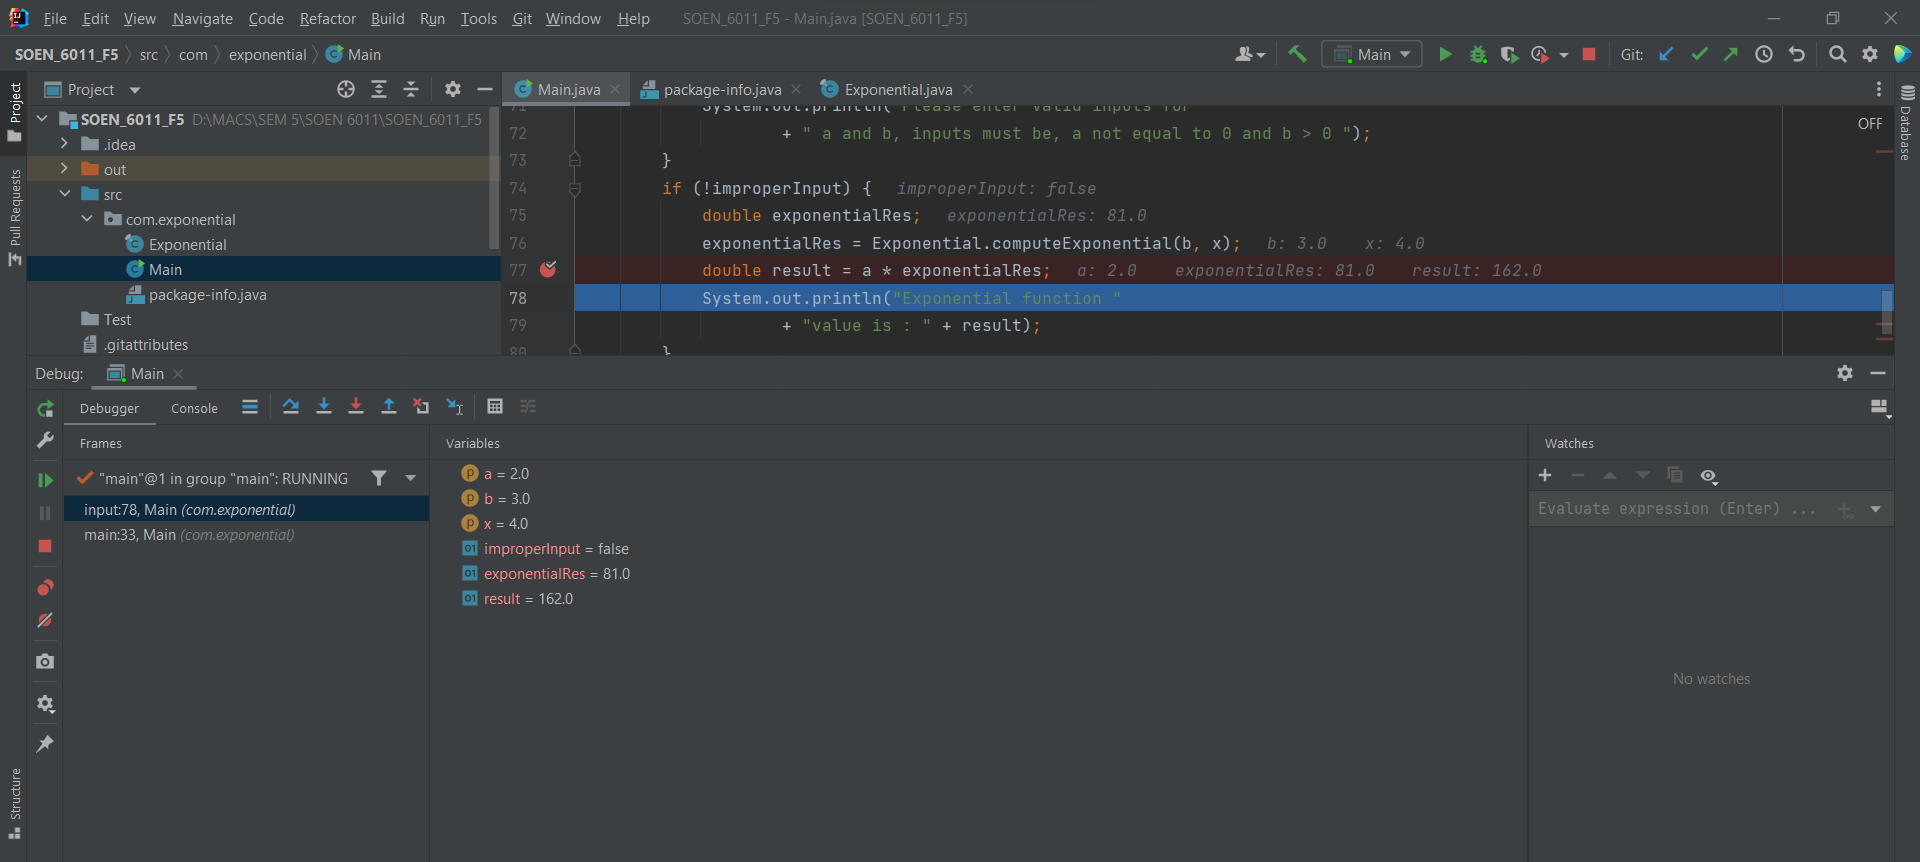
\includegraphics[width=15cm,height=9cm]{debugger-1.png}
  \caption{Debugging computation of exponential function}
  \label{fig:Debugging computation of exponential function}
\end{figure}


\begin{figure}[h!]
  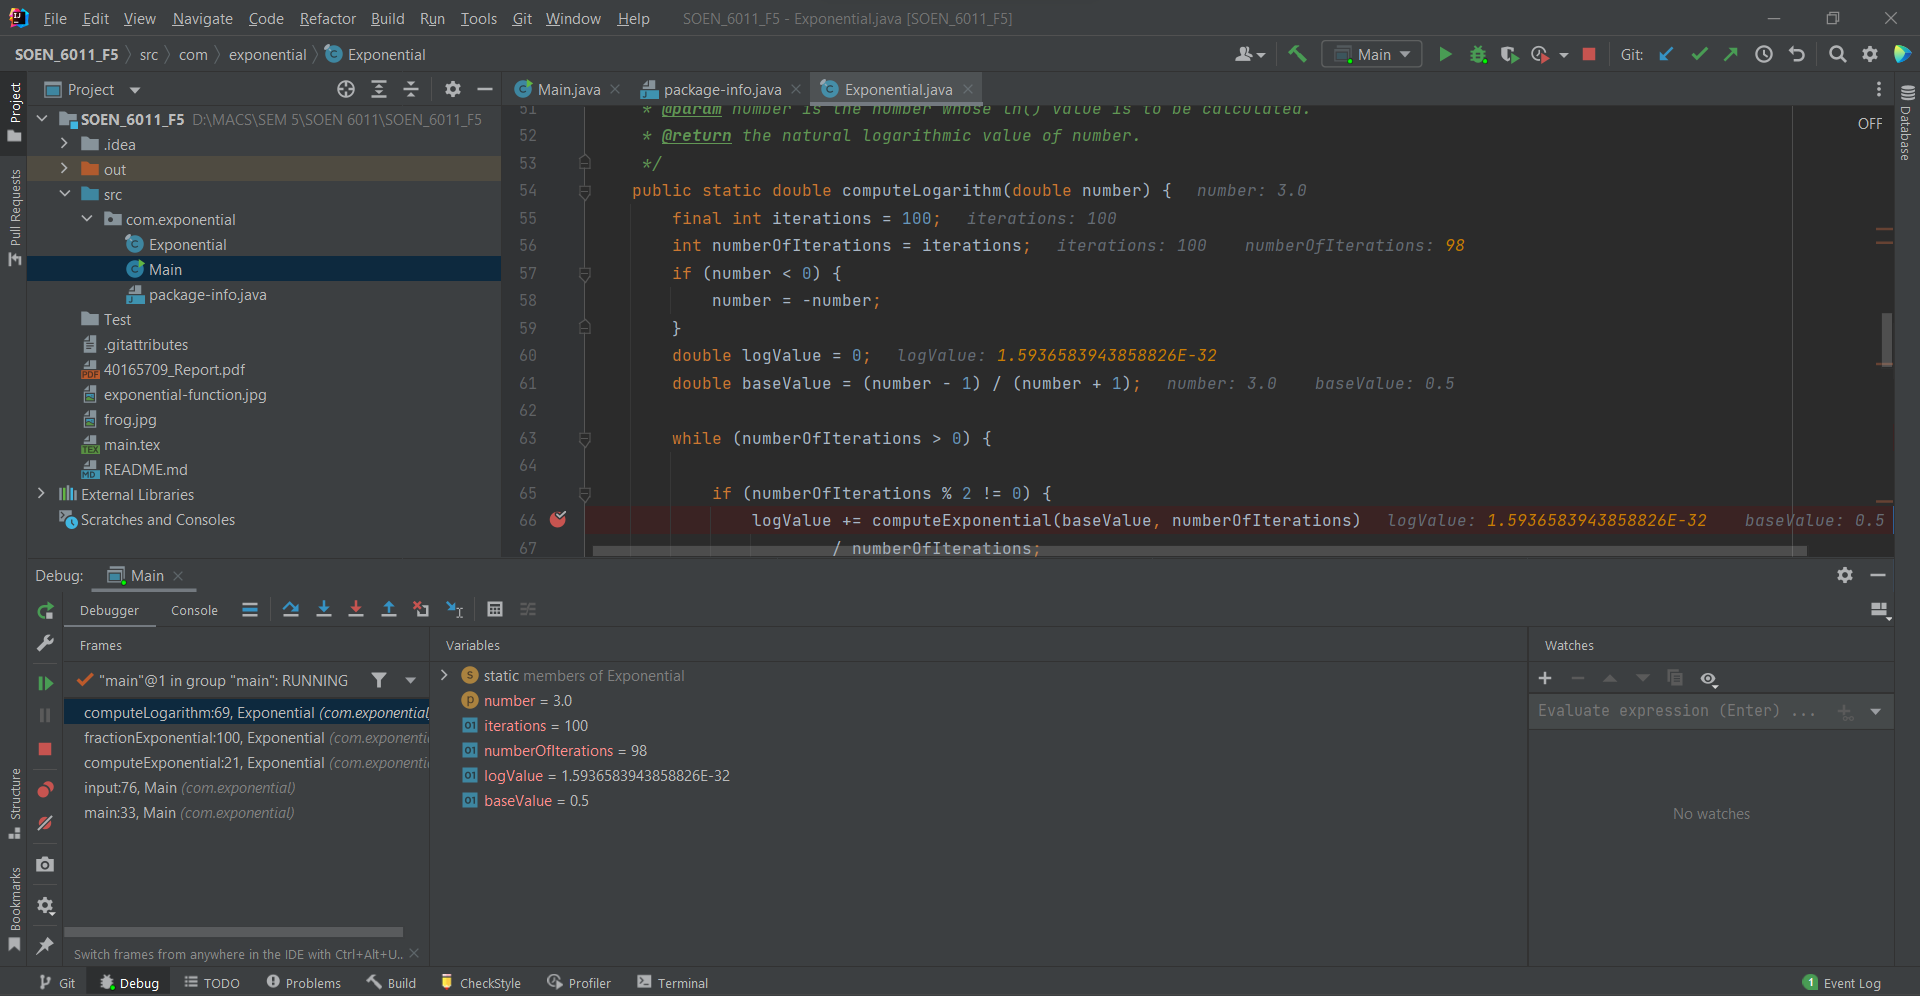
\includegraphics[width=15cm,height=9cm]{debugger-2.png}
  \caption{Debugging computation of fractional exponent value}
  \label{Debugging computation of fractional exponent value}
\end{figure}

\newpage

\newpage

\subsection{Quality Attributes}
This section highlights and describes several efforts made to achieve the desired quality attributes related to the java program .
\begin{enumerate}
    \item \textbf{Efficient} – The program uses recursive algorithm to compute the exponential value and it provides time complexity of $O(logn)$ and it is the same for space complexity due to recursive stack space. It is more efficient and better choice in comparison to other approaches. As a result, the program runs quickly, and the function value is computed within required time window.
    \item \textbf{Maintainable} – The program is partitioned into various methods each responsible for certain kind of computation, I have divided the user interface, error handling part $(Main.java)$ from the core logic part $(Exponential.java)$ related to the calculation of exponential function value. It allows easy modification of features/functionalities as well as adding new ones. It makes the code maintainable.
    \item \textbf{Correctness} – I have designed several test cases to check the program against all the possible values of the base and exponent including invalid inputs, fractional exponent, negative exponents, every test case successfully runs and hence the developed program provides correct results and agrees to the desired specifications.
    \item \textbf{Robust} – Input values are validated as they are entered by the user and all the invalid inputs are rejected. On entering such inputs, the program displays corresponding error message and asks for new valid input values from the user. In this way error handling is performed to avoid any kind of failure. 
    \item \textbf{Usable} – The program provides text-based user interface to the user for entering the values and displays the computed result. The error messages are meaningful and can be easily understood. It provides functionality for user to continue the computation for other values or exit the system. In this way, the program is made user-friendly.
    \item \textbf{Portable} - The program is developed in java language, so it can be executed on other platforms as well as systems without requiring any modifications. 
\end{enumerate}

\newpage

\end{document}